% =============================================================================
% Section 3: Experimental Design
% =============================================================================
\section{Experimental Design}
\label{sec:experimental_design}

This section presents the complete experimental protocol as a unified, replicable specification.  Every design choice is stated with its rationale.  A reader equipped with the accompanying repository can reproduce every reported number by following this section sequentially.

% --------------------------------------------------------------------------
\subsection{Formal Problem Definition}
\label{sec:problem_definition}

Let $\bX_t \in \R^{w \times d}$ denote a multivariate input window of $w$ consecutive hourly observations with $d = 5$ OHLCV features (Open, High, Low, Close, Volume), ending at time index~$t$.  The forecasting task is to learn a parametric mapping
\begin{equation}
  f_{\btheta}: \R^{w \times d} \rightarrow \R^{h},
  \quad \byhat_{t+1:t+h} = f_{\btheta}(\bX_t),
  \quad h \in \{4, 24\},
  \label{eq:task}
\end{equation}
where $\byhat_{t+1:t+h}$ is the predicted vector of future Close prices and $\btheta$ collects all learnable parameters.  Two horizon configurations are evaluated as \emph{completely separate experiments}, with no shared weights or intermediate results:

\begin{itemize}[nosep]
  \item \textbf{Short-term} ($\hfour$): lookback window $w = 24$ hours, predicting 4 hours ahead.
  \item \textbf{Long-term} ($\htwentyfour$): lookback window $w = 96$ hours, predicting 24 hours ahead.
\end{itemize}

All models employ \emph{direct multi-step forecasting}: the entire horizon vector $\byhat \in \R^h$ is produced in a single forward pass.  No model feeds predictions back as inputs, avoiding the error accumulation of recursive strategies \citep{Taieb2012, Chevillon2007}.  The training objective is mean squared error:
\begin{equation}
  \mathcal{L}(\btheta) = \frac{1}{n} \sum_{i=1}^{n} \|\by_i - \byhat_i\|^2,
  \label{eq:loss}
\end{equation}
and the model selection criterion is minimum validation \mse.  This common loss function and selection criterion apply identically to all architectures, eliminating confounds from differential training objectives.

% --------------------------------------------------------------------------
\subsection{Data}
\label{sec:data}

\subsubsection{Asset Universe}
\label{sec:asset_universe}

The benchmark spans \nassets financial instruments across three asset classes, each with structurally distinct market microstructure:

\begin{itemize}
  \item \textbf{Cryptocurrency} (4 assets): BTC/USDT, ETH/USDT, BNB/USDT, ADA/USDT.  These instruments trade continuously (24/7), exhibit high volatility, and are subject to rapid regime changes driven by speculative activity and regulatory events.

  \item \textbf{Forex} (4 assets): EUR/USD, USD/JPY, GBP/USD, AUD/USD.  Major currency pairs are characterised by high liquidity, short-term mean-reverting tendencies, and sensitivity to macroeconomic announcements and central-bank policy.

  \item \textbf{Equity indices} (4 assets): Dow Jones, S\&P 500, NASDAQ 100, DAX.  These indices track broad equity markets, exhibiting trending behaviour, lower intra-day volatility relative to cryptocurrency, and session-based trading hours.
\end{itemize}

All instruments are sampled at H1 (1-hour) frequency, providing uniform temporal resolution across asset classes.  For hyperparameter optimisation, one representative asset per class is designated: BTC/USDT (cryptocurrency), EUR/USD (forex), and Dow Jones (equity indices).  Optimised configurations are frozen and applied to all assets within the corresponding class, preventing asset-level overfitting while preserving category-level calibration (Section~\ref{sec:stage2_freeze}).

\subsubsection{Feature Specification}
\label{sec:feature_spec}

All models receive identical input tensors comprising five raw market features: Open, High, Low, Close, and Volume (OHLCV).  This deliberate restriction to unprocessed market data isolates the contribution of architectural design from feature-engineering confounds.  No technical indicators, lagged returns, calendar variables, or external covariates are introduced.  The sole forecast target is the Close price at each horizon step, ensuring that performance differences reflect architecture rather than feature availability.

\subsubsection{Preprocessing}
\label{sec:preprocessing}

The preprocessing pipeline transforms raw market data into normalised, windowed tensors through four stages:

\begin{enumerate}
  \item \textbf{Loading.}  Raw hourly OHLCV records are ingested from CSV files containing datetime, open, high, low, close, and volume columns.

  \item \textbf{Truncation.}  To ensure comparable dataset sizes across instruments with different histories, the most recent 30{,}000 time steps are retained for every asset prior to windowing.

  \item \textbf{Normalisation.}  Standard $z$-score normalisation (zero mean, unit variance) is fitted \emph{exclusively on the training partition} and applied unchanged to validation and test partitions.  This prevents leakage of future distributional information into the scaling statistics.  After inference, predictions are inverse-scaled to the original price domain before metric computation.

  \item \textbf{Windowing.}  Rolling windows of length $w + h$ are constructed.  Two configurations are employed: $(w, h) = (24, 4)$ for short-term and $(w, h) = (96, 24)$ for long-term forecasting.  Each window yields an input matrix $\bX \in \R^{w \times 5}$ and a target vector $\by \in \R^{h}$ (Close prices only).
\end{enumerate}

\subsubsection{Chronological Splits}
\label{sec:splits}

All partitions are strictly chronological to prevent future-data leakage:
\begin{itemize}[nosep]
  \item \textbf{Training}: first 70\% of samples (approximately 21{,}000 windows per asset per horizon).
  \item \textbf{Validation}: next 15\% of samples (approximately 4{,}500 windows).
  \item \textbf{Test}: final 15\% of samples (approximately 4{,}500 windows).
\end{itemize}

No shuffling is performed at any stage, preserving the temporal ordering essential for financial time-series.  Identical splits are applied to all models, ensuring that every architecture receives exactly the same training, validation, and test observations for each (asset, horizon) pair.  Split boundaries and sample counts are recorded alongside the processed datasets (Table~\ref{tab:dataset_summary}).  Return distributional statistics---mean return, volatility, skewness, excess kurtosis, first-order autocorrelation, and ADF unit-root test \pvalue---for all twelve assets are reported in Table~\ref{tab:distributional_stats}; all return series are stationary ($p < 0.001$) with heavy tails (excess kurtosis 15--96) and near-zero mean returns consistent with weak-form market efficiency.

% =============================================================================
% Table 2: Dataset Summary
% =============================================================================
\begin{table}[htbp]
  \centering
  \caption{Dataset summary.  All assets use H1 (hourly) frequency.  The most
    recent 30{,}000 windowed samples are retained per (asset, horizon) pair,
    split chronologically into 70\%/15\%/15\% train/val/test partitions.
    Window lengths: $w=24$ for $h=4$ and $w=96$ for $h=24$.  Features: OHLCV
    (5 channels); target: close price.}
  \label{tab:dataset_summary}
  \setlength{\tabcolsep}{6pt}%
  \begin{tabular}{%
    l%          Category
    l%          Asset
    l%          Date Range
    r%          Train
    r%          Val
    r%          Test
    r%          Total
  }
    \toprule
    \textbf{Category} & \textbf{Asset} & \textbf{Date Range}
      & \textbf{Train} & \textbf{Val} & \textbf{Test} & \textbf{Total} \\
    \midrule
    \multirow{4}{*}{Crypto}
      & BTC/USDT  & 2021-03 -- 2026-02 & 21{,}000 & 4{,}500 & 4{,}500 & 30{,}000 \\
      & ETH/USDT  & 2021-03 -- 2026-02 & 21{,}000 & 4{,}500 & 4{,}500 & 30{,}000 \\
      & BNB/USDT  & 2021-03 -- 2026-02 & 21{,}000 & 4{,}500 & 4{,}500 & 30{,}000 \\
      & ADA/USDT  & 2021-05 -- 2026-02 & 21{,}000 & 4{,}500 & 4{,}500 & 30{,}000 \\
    \midrule
    \multirow{4}{*}{Forex}
      & EUR/USD   & 2017-12 -- 2026-02 & 21{,}000 & 4{,}500 & 4{,}500 & 30{,}000 \\
      & USD/JPY   & 2017-12 -- 2026-02 & 21{,}000 & 4{,}500 & 4{,}500 & 30{,}000 \\
      & GBP/USD   & 2017-12 -- 2026-02 & 21{,}000 & 4{,}500 & 4{,}500 & 30{,}000 \\
      & AUD/USD   & 2017-12 -- 2026-02 & 21{,}000 & 4{,}500 & 4{,}500 & 30{,}000 \\
    \midrule
    \multirow{4}{*}{Indices}
      & Dow Jones   & 2019-01 -- 2026-02 & 21{,}000 & 4{,}500 & 4{,}500 & 30{,}000 \\
      & S\&P~500    & 2019-01 -- 2026-02 & 21{,}000 & 4{,}500 & 4{,}500 & 30{,}000 \\
      & NASDAQ~100  & 2019-01 -- 2026-02 & 21{,}000 & 4{,}500 & 4{,}500 & 30{,}000 \\
      & DAX         & 2019-02 -- 2026-02 & 21{,}000 & 4{,}500 & 4{,}500 & 30{,}000 \\
    \midrule
    \multicolumn{2}{l}{\textbf{Total per horizon}} & ---
      & 252{,}000 & 54{,}000 & 54{,}000 & 360{,}000 \\
    \bottomrule
  \end{tabular}
\end{table}

% =============================================================================
% Table 2b: Distributional Statistics per Asset
% =============================================================================
\begin{table}[htbp]
  \centering
  \caption{Distributional statistics of hourly log returns for all twelve
    assets.  All series reject the Augmented Dickey--Fuller unit-root null
    at $p < 0.001$, confirming return stationarity.}
  \label{tab:distributional_stats}
  \setlength{\tabcolsep}{5pt}%
  \begin{threeparttable}
  \begin{tabular}{%
    l%          Category
    l%          Asset
    r%          Mean return (x1e-4)
    r%          Volatility (%)
    r%          Skewness
    r%          Kurtosis
    r%          ACF(1)
    l%          ADF p-value
  }
    \toprule
    \textbf{Cat.} & \textbf{Asset}
      & $\bar{\mu}_r$ (${\times}10^{-4}$)
      & $\sigma_r$ (\%)
      & Skew
      & Kurt
      & ACF(1)
      & ADF $p$ \\
    \midrule
    \multirow{4}{*}{Crypto}
      & BTC/USDT  & $+0.4$ & 0.783 & $-0.47$ & $+35.8$ & $-0.043$ & $<$0.001 \\
      & ETH/USDT  & $+0.3$ & 0.973 & $-0.56$ & $+27.3$ & $-0.026$ & $<$0.001 \\
      & BNB/USDT  & $+0.8$ & 1.107 & $+0.08$ & $+35.0$ & $-0.077$ & $<$0.001 \\
      & ADA/USDT  & $\phantom{+}0.0$ & 1.187 & $-0.05$ & $+19.2$ & $-0.085$ & $<$0.001 \\
    \midrule
    \multirow{4}{*}{Forex}
      & EUR/USD   & $\phantom{+}0.0$ & 0.109 & $-0.01$ & $+15.2$ & $-0.010$ & $<$0.001 \\
      & USD/JPY   & $+0.1$ & 0.119 & $-0.98$ & $+46.6$ & $-0.002$ & $<$0.001 \\
      & GBP/USD   & $\phantom{+}0.0$ & 0.115 & $-1.66$ & $+95.8$ & $-0.018$ & $<$0.001 \\
      & AUD/USD   & $\phantom{+}0.0$ & 0.141 & $-0.07$ & $+17.9$ & $-0.020$ & $<$0.001 \\
    \midrule
    \multirow{4}{*}{Indices}
      & Dow Jones   & $+0.2$ & 0.225 & $-0.57$ & $+60.8$ & $-0.012$ & $<$0.001 \\
      & S\&P~500    & $+0.2$ & 0.235 & $-1.13$ & $+90.2$ & $-0.026$ & $<$0.001 \\
      & NASDAQ~100  & $+0.3$ & 0.286 & $-0.70$ & $+47.7$ & $-0.014$ & $<$0.001 \\
      & DAX         & $+0.2$ & 0.262 & $-1.74$ & $+83.0$ & $-0.011$ & $<$0.001 \\
    \bottomrule
  \end{tabular}
  \begin{tablenotes}[flushleft]\small
    \item All return distributions exhibit excess kurtosis (heavy tails) consistent with the
    stylised facts of financial markets; equities and forex show negative skewness (downside
    asymmetry), while crypto skewness is near zero.  Negative ACF(1) values indicate
    mild mean-reversion in hourly returns.  Volatility spans two orders of magnitude
    across asset classes (crypto $\approx 1\%$, forex $\approx 0.1\%$, indices $\approx 0.2\%$),
    reflecting differences in leverage, liquidity, and trading hours.
  \end{tablenotes}
  \end{threeparttable}
\end{table}


% Sample data figure
\begin{figure}[htbp]
  \centering
  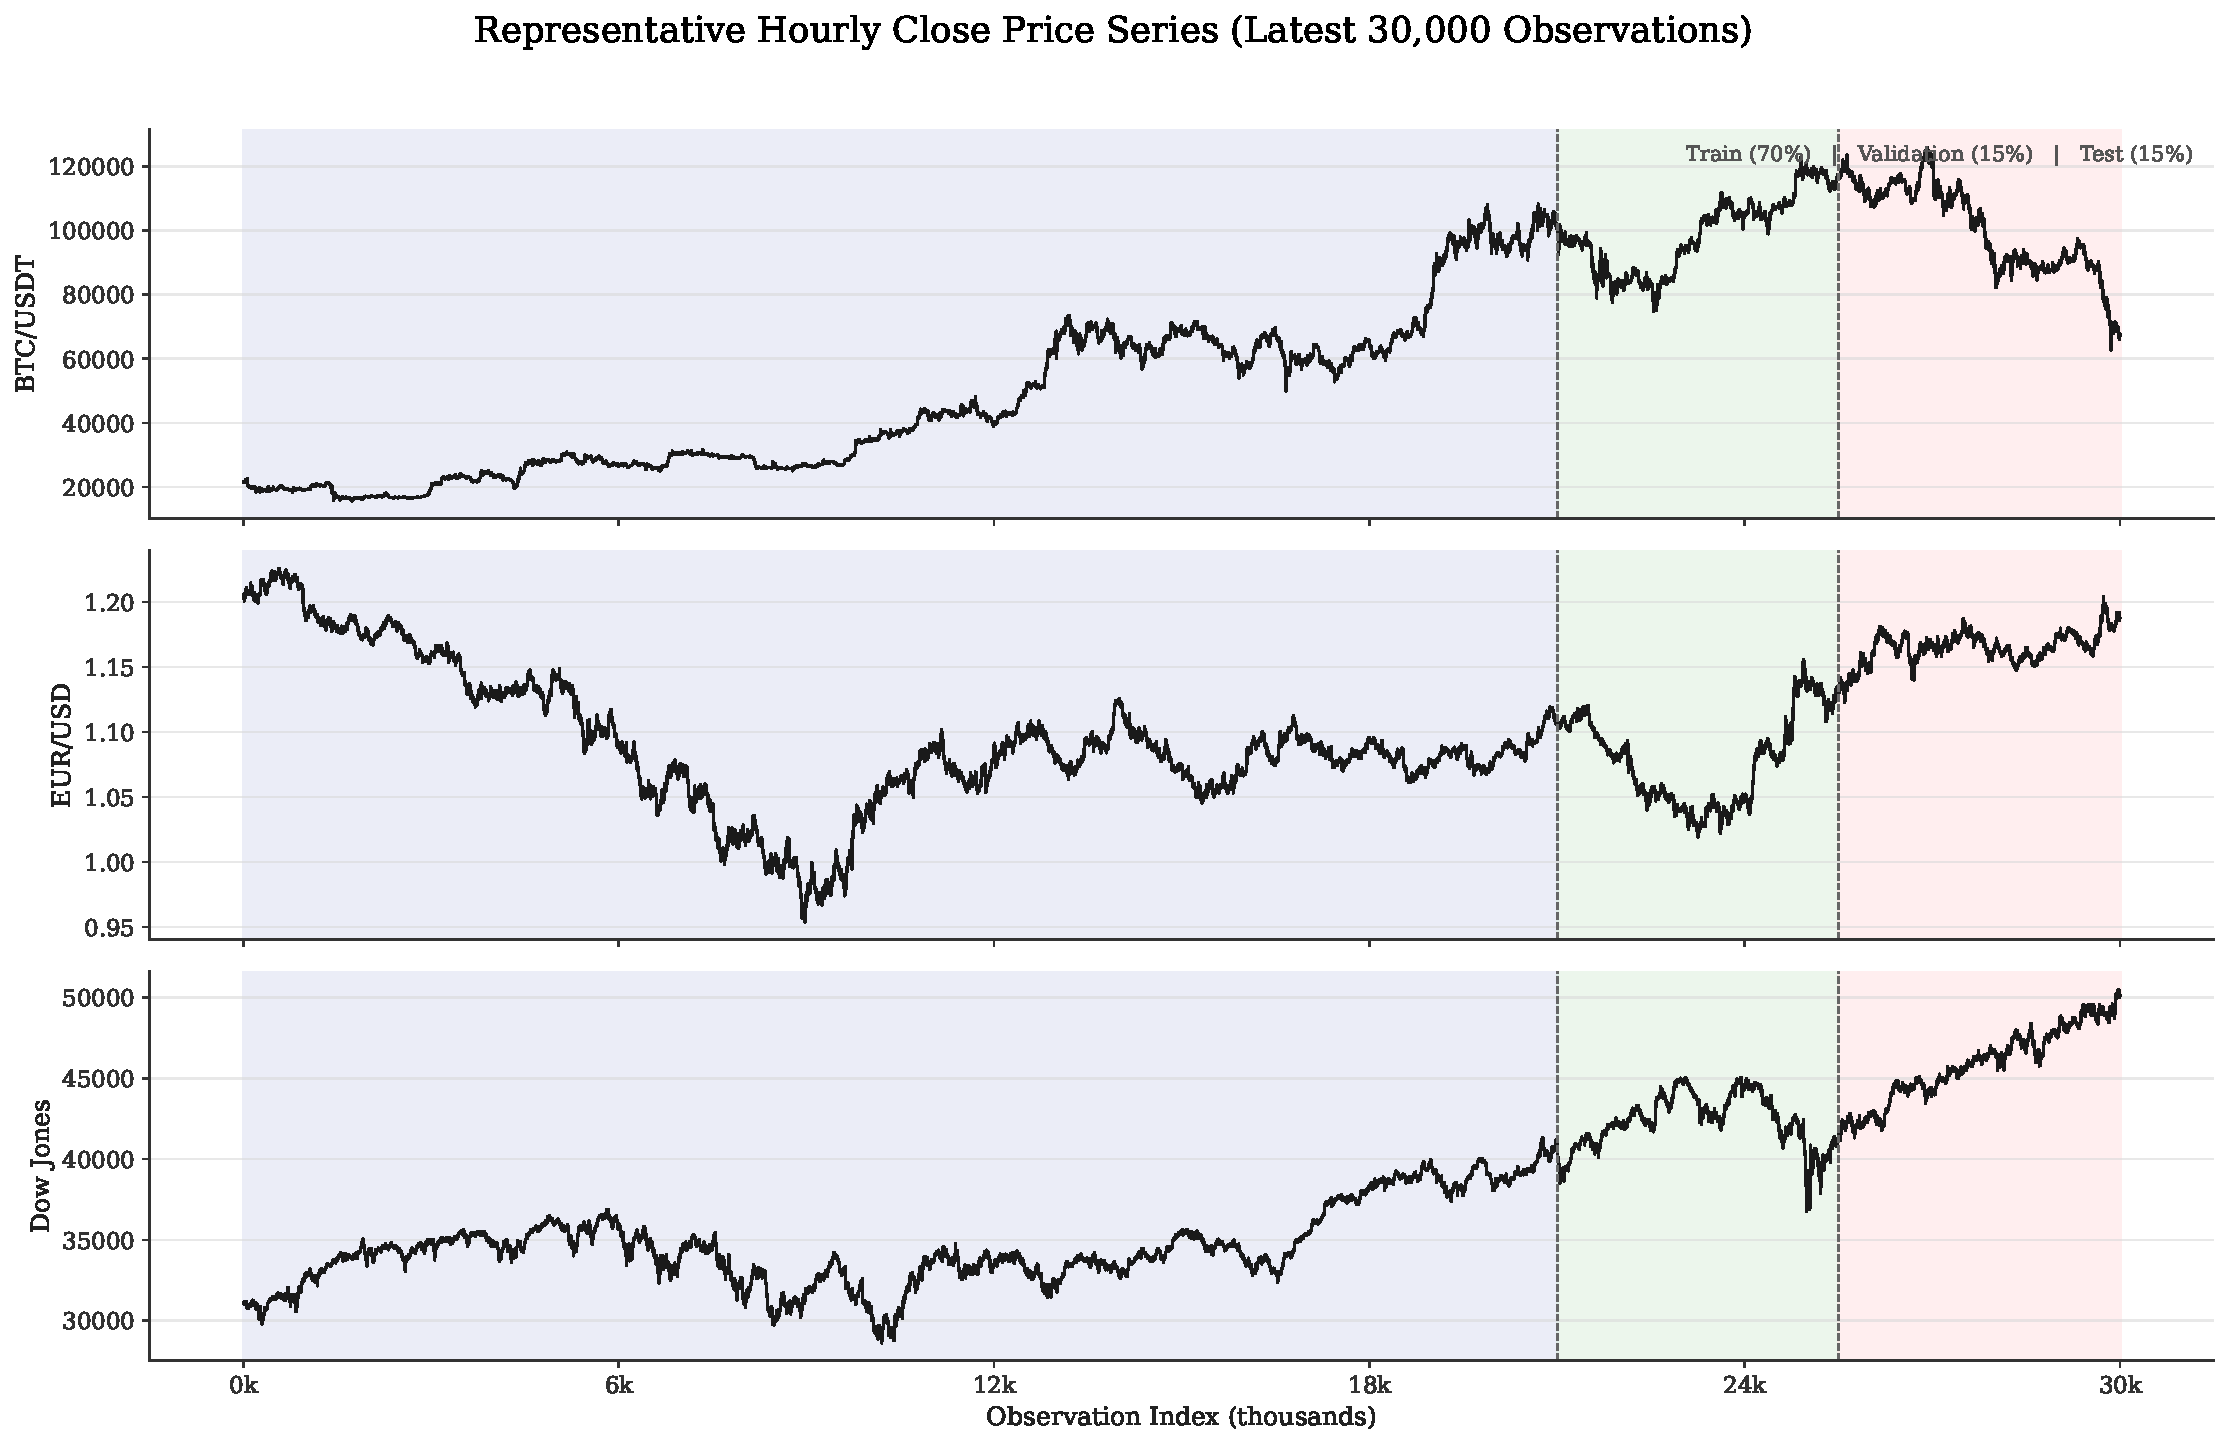
\includegraphics[width=\textwidth]{figures/01_sample_data.pdf}
  \caption{Representative hourly Close-price time series for one asset per class: BTC/USDT (cryptocurrency), EUR/USD (forex), and Dow Jones (equity indices).  Vertical dashed lines indicate chronological train/validation/test boundaries (70/15/15 split).  The three classes exhibit qualitatively different dynamics: high-volatility trending behaviour (cryptocurrency), low-volatility mean-reversion around a narrow range (forex), and moderate-volatility upward drift (equity indices).  All series comprise the most recent 30{,}000 hourly observations.}
  \label{fig:sample_data}
\end{figure}

% --------------------------------------------------------------------------
\subsection{Model Architectures}
\label{sec:model_architectures}

\Nmodels architectures spanning four families are evaluated.  All models conform to a unified interface: input shape $(B, w, d)$ with $d = 5$ OHLCV features; output shape $(B, h)$, where $B$ is the batch size.  No model-specific feature engineering or data augmentation is permitted.  Table~\ref{tab:model_architectures} summarises the key architectural properties.

\paragraph{Transformer family (4 models).}
\autoformer \citep{Wu2021} replaces self-attention with an auto-correlation mechanism operating in the frequency domain at $\bigO(L \log L)$ complexity, incorporating progressive series decomposition to separate trend and seasonal components.

\patchtst \citep{Nie2023} segments input series into patches, treats each as a token, and applies a Transformer encoder with channel-independent processing and RevIN normalisation \citep{Kim2022}.

\itransformer \citep{Liu2024itransformer} inverts the attention paradigm: each variate's full temporal trajectory serves as a token, and attention is computed across the variate dimension.

\timexer \citep{Wang2024timexer} separates target and exogenous variables, embedding patched target representations alongside learnable global tokens and applying cross-attention to query inverted exogenous embeddings.

\paragraph{MLP/linear family (2 models).}
\dlinear \citep{Zeng2023} applies moving-average decomposition to separate seasonal and trend components, then maps each through an independent linear layer---without hidden layers, activations, or attention.  It has the fewest parameters of any model in the benchmark (approximately 1{,}000 at $\hfour$).

\nhits \citep{Challu2023} employs a hierarchical stack of MLP blocks with multi-rate pooling.  Each block operates at a different temporal resolution and interpolates coefficients to the forecast horizon through basis-function expansion.

\paragraph{Convolutional family (2 models).}
\timesnet \citep{Wu2023timesnet} transforms forecasting from 1D to 2D by identifying dominant FFT-based periods, reshaping the sequence into 2D tensors, and applying Inception-style 2D convolutions to capture intra-period and inter-period patterns.

\moderntcn \citep{Luo2024moderntcn} employs large-kernel depthwise convolutions with structural reparameterisation, multi-stage downsampling, and optional RevIN normalisation for multi-scale temporal pattern extraction.

\paragraph{Recurrent family (1 model).}
\lstm \citep{Hochreiter1997} serves as the classical baseline: a multi-layer stacked LSTM encoder extracts the final hidden state, which a two-layer MLP head projects to the forecast vector.

% =============================================================================
% Table 3: Model Architectures
% =============================================================================
\begin{table}[htbp]
  \centering
  \caption{Summary of the nine deep learning architectures evaluated.  All
    models receive OHLCV input of shape $(B,\,w,\,5)$ and produce direct
    multi-step forecasts of shape $(B,\,h)$.  Family abbreviations:
    RNN~= recurrent, MLP~= multi-layer perceptron,
    TCN~= temporal convolutional network, TF~= Transformer.}
  \label{tab:model_architectures}
  \small
  \setlength{\tabcolsep}{4pt}%
  \begin{tabular}{%
    l%          Model
    c%          Family
    p{5.5cm}%   Key Mechanism
    l%          Reference
  }
    \toprule
    \textbf{Model} & \textbf{Family} & \textbf{Key Mechanism} & \textbf{Reference} \\
    \midrule
    \autoformer   & TF  & Auto-correlation \& series decomposition        & \citep{Wu2021} \\
    \dlinear      & MLP & Linear layers with trend--seasonal decomposition & \citep{Zeng2023} \\
    \itransformer & TF  & Inverted attention on variate tokens             & \citep{Liu2024itransformer} \\
    \lstm         & RNN & Gated recurrent cells + dense MLP projection head & \citep{Hochreiter1997} \\
    \moderntcn    & TCN & Large-kernel depthwise convolutions with patching & \citep{Luo2024moderntcn} \\
    \nhits        & MLP & Hierarchical interpolation with multi-rate pooling & \citep{Challu2023} \\
    \patchtst     & TF  & Channel-independent patch-based Transformer      & \citep{Nie2023} \\
    \timesnet     & TCN & 2D temporal variation via FFT + Inception blocks  & \citep{Wu2023timesnet} \\
    \timexer      & TF  & Exogenous-variable-aware cross-attention          & \citep{Wang2024timexer} \\
    \bottomrule
  \end{tabular}
\end{table}


% --------------------------------------------------------------------------
\subsection{Five-Stage Experimental Pipeline}
\label{sec:pipeline}

The experimental pipeline comprises five sequential stages, each designed to eliminate a specific source of confounding.  Figure~\ref{fig:pipeline} provides a schematic overview.

\subsubsection{Stage 1: Fixed-Seed Hyperparameter Optimisation}
\label{sec:stage1_hpo}

Hyperparameter optimisation is performed using the Optuna framework \citep{Akiba2019} with the Tree-structured Parzen Estimator (TPE) sampler \citep{Bergstra2011}.  To ensure fairness, the following settings are held constant across all architectures:

\begin{itemize}[nosep]
  \item \textbf{Deterministic seed:} 42 (identical random state for all HPO runs).
  \item \textbf{Trial budget:} \ntrials trials per (model, category, horizon) configuration.
  \item \textbf{Sampler:} TPE with median pruner (2 startup trials, 5 warm-up steps).
  \item \textbf{Objective:} Minimise validation \mse.
  \item \textbf{Training budget per trial:} 50 epochs, batch size~256.
\end{itemize}

HPO is conducted exclusively on one representative asset per category (BTC/USDT, EUR/USD, Dow Jones), preventing overfitting to individual assets while capturing category-level dynamics.  This design is motivated by two considerations: (i)~tuning on all 12 assets would multiply computational cost by $12\times$ without a mechanism for cross-asset generalisation, and (ii)~freezing configurations at the category level ensures the same inductive prior governs all assets within a class.  Table~\ref{tab:hpo_search_spaces} provides the full search space specification.

The controlled \ntrials-trial budget is a deliberate choice that prioritises comparative fairness over exhaustive peak-performance search.  Three considerations justify this constraint.  First, in financial time-series forecasting---where the signal-to-noise ratio is low and non-stationarity is pervasive---extensive HPO risks selecting configurations that overfit to transient market regimes and fail to generalise to the test set.  To mitigate this risk, search ranges were drawn from commonly used configurations in the literature, and identical budgets were applied to all models to ensure a symmetrical evaluation framework.

Second, model parameter counts were kept in a comparable range across architectures (with the exception of \dlinear, which is intentionally lightweight by design).  Maintaining comparable capacity reduces search-space imbalance and prevents capacity-driven advantages from confounding the architectural comparison.

Third, the empirical evidence corroborates this design: the variance decomposition and rank stability across horizons (Section~\ref{sec:results}) show that architectural identity is the dominant factor in performance variance, and the high consistency of model rankings suggests that an expanded HPO budget would yield diminishing returns unlikely to alter the comparative conclusions.  Consequently, this protocol prioritises cross-architectural fairness and statistical validity, ensuring that observed performance differences reflect structural merits rather than differential tuning intensity.

% =============================================================================
% Table 4: HPO Search Spaces (Summary)
% =============================================================================
\begin{table}[htbp]
  \centering
  \caption{Hyperparameter search spaces per model.  All models share learning
    rate $\in [5\times10^{-4},\,5\times10^{-3}]$ (log-uniform) and batch
    size $\in\{64,128\}$.  Only architecture-specific parameters are shown.
    HPO uses Optuna TPE with \ntrials trials per (model $\times$ horizon
    $\times$ asset class) on representative assets (BTC/USDT, EUR/USD,
    Dow Jones) only.}
  \label{tab:hpo_search_spaces}
  \small
  \setlength{\tabcolsep}{6pt}%
  \renewcommand{\arraystretch}{0.92}%
  \begin{tabular}{%
    l%          Model
    l%          Hyperparameter
    p{5.2cm}%   Range / Choices
  }
    \toprule
    \textbf{Model} & \textbf{Hyperparameter} & \textbf{Range / Choices} \\
    \midrule
    \multirow{5}{*}{\autoformer}
      & Model dimension          & $\{64, 128\}$ \\
      & Attention heads          & $\{4, 8\}$ \\
      & Enc./dec.\ layers        & $\{1, 2\}$ each \\
      & Feedforward dimension    & $\{64, 128\}$ \\
      & Dropout rate             & $[0.0, 0.2]$, step~$0.05$ \\
    \midrule
    \multirow{2}{*}{\dlinear}
      & Moving-average kernel    & $[3, 51]$, step~$2$ \\
      & Per-channel mapping      & $\{\text{true}, \text{false}\}$ \\
    \midrule
    \multirow{4}{*}{\itransformer}
      & Model dimension          & $\{96, 112\}$ \\
      & Feedforward dimension    & $\{128, 256\}$ \\
      & Encoder layers           & $[2, 4]$ \\
      & Attention heads          & $\{4, 8, 16\}$ \\
    \midrule
    \multirow{4}{*}{\lstm}
      & Hidden state size        & $\{64, 128\}$ \\
      & Recurrent layers         & $[1, 3]$ \\
      & Projection head width    & $\{64, 128\}$ \\
      & Bidirectional            & $\{\text{true}, \text{false}\}$ \\
    \midrule
    \multirow{4}{*}{\moderntcn}
      & Patch size               & $\{8, 16\}$ \\
      & Channel dimensions       & $[32, 64, 96]$ \\
      & RevIN normalisation      & $\{\text{true}, \text{false}\}$ \\
      & Dropout / head dropout  & $[0.0, 0.2]$, step~$0.05$ \\
    \midrule
    \multirow{4}{*}{\nhits}
      & Number of blocks         & $[2, 3]$ \\
      & Hidden layer width       & $\{64, 96\}$ \\
      & Layers per block         & $[3, 6]$ \\
      & Pooling kernel sizes     & $\{[2,4,8],\,[4,8,12]\}$ \\
    \midrule
    \multirow{4}{*}{\patchtst}
      & Model dimension          & $\{64\}$ \\
      & Encoder layers           & $[1, 3]$ \\
      & Patch length             & $\{16, 24\}$ \\
      & Stride                   & $\{4, 8\}$ \\
    \midrule
    \multirow{3}{*}{\timesnet}
      & Model dimension          & $\{24, 32\}$ \\
      & Feedforward dimension    & $\{32, 64\}$ \\
      & Encoder layers           & $[2, 3]$ \\
    \midrule
    \multirow{4}{*}{\timexer}
      & Model dimension          & $\{64, 96\}$ \\
      & Feedforward dimension    & $\{128, 256\}$ \\
      & Encoder layers           & $[2, 3]$ \\
      & Attention heads          & $\{4, 8\}$ \\
    \bottomrule
  \end{tabular}
\end{table}


\subsubsection{Stage 2: Configuration Freezing}
\label{sec:stage2_freeze}

The best-performing configuration for each (model, category, horizon) triple---determined by validation \mse in Stage~1---is recorded and frozen.  These frozen configurations are applied unchanged to all assets within the corresponding category; no further tuning is permitted.  This eliminates asset-level overfitting and ensures that each architecture is evaluated on a single, category-level configuration.  Table~\ref{tab:best_hyperparameters} presents the selected configurations.

% =============================================================================
% Table 5: Best Hyperparameters (Frozen after HPO)
% =============================================================================
\begin{table}[htbp]
  \centering
  \caption{Frozen best hyperparameters selected via Optuna TPE (\ntrials
    trials, seed~42, objective: minimum validation \mse).  Only key
    architecture-specific parameters are shown; all configurations also
    include learning rate and batch size.  Shared entries across categories
    indicate that the representative-asset optimum was identical.}
  \label{tab:best_hyperparameters}
  \footnotesize
  \setlength{\tabcolsep}{5pt}%
  \resizebox{\textwidth}{!}{%
  \begin{tabular}{%
    l%          Model
    l%          Category
    c%          Horizon
    p{8cm}%     Key Parameters
  }
    \toprule
    \textbf{Model} & \textbf{Category} & \textbf{$h$} & \textbf{Key Parameters} \\
    \midrule
    \multirow{2}{*}{\autoformer}
      & Crypto/Forex & 4/24 & $d_{\mathrm{model}}{=}128$, heads${=}4$, enc${=}1$, dec${=}2$, $d_{\mathrm{ff}}{=}128$, drop${=}0.20$ \\
      & Indices      & 4/24 & $d_{\mathrm{model}}{=}128$, heads${=}4$, enc${=}1$, dec${=}2$, $d_{\mathrm{ff}}{=}128$, drop${=}0.10$ \\
    \midrule
    \multirow{2}{*}{\dlinear}
      & All          & 4    & kernel${=}21$, individual${=}\text{true}$ \\
      & Crypto/Forex & 24   & kernel${=}43$, individual${=}\text{true}$ \\
    \midrule
    \multirow{2}{*}{\itransformer}
      & Crypto       & 24   & $d_{\mathrm{model}}{=}112$, $d_{\mathrm{ff}}{=}128$, layers${=}2$, heads${=}16$, drop${=}0.15$ \\
      & Other        & 4    & $d_{\mathrm{model}}{=}96$,  $d_{\mathrm{ff}}{=}128$, layers${=}4$, heads${=}16$, drop${=}0.00$ \\
    \midrule
    \multirow{2}{*}{\lstm}
      & All          & 4    & hidden${=}128$, layers${=}1$, mlp${=}128$, bidir${=}\text{true}$, drop${=}0.15$ \\
      & All          & 24   & hidden${=}64$,  layers${=}1$, mlp${=}128$, bidir${=}\text{true}$, drop${=}0.10$ \\
    \midrule
    \multirow{2}{*}{\moderntcn}
      & Crypto       & 24   & patch${=}16$, dims${=}[32,64,96]$, RevIN, drop${=}0.20$, head-drop${=}0.20$ \\
      & Other        & 4/24 & patch${=}8$,  dims${=}[32,64,96]$, RevIN+affine, drop${=}0.10$, head-drop${=}0.10$ \\
    \midrule
    \multirow{2}{*}{\nhits}
      & Crypto       & 4    & blocks${=}2$, hidden${=}64$, layers${=}3$, pool${=}[4,8,12]$, drop${=}0.05$ \\
      & Crypto       & 24   & blocks${=}3$, hidden${=}96$, layers${=}4$, pool${=}[4,8,12]$, drop${=}0.00$ \\
    \midrule
    \multirow{2}{*}{\patchtst}
      & Crypto       & 4    & $d_{\mathrm{model}}{=}64$, layers${=}2$, patch${=}24$, stride${=}8$, drop${=}0.05$ \\
      & Other        & 24   & $d_{\mathrm{model}}{=}64$, layers${=}1$, patch${=}24$, stride${=}4$, drop${=}0.15$ \\
    \midrule
    \timesnet
      & All          & 4/24 & $d_{\mathrm{model}}{=}32$, $d_{\mathrm{ff}}{=}32$, layers${=}2$, top-$k{=}3$, drop${=}0.00$ \\
    \midrule
    \multirow{2}{*}{\timexer}
      & Crypto       & 4    & $d_{\mathrm{model}}{=}64$, $d_{\mathrm{ff}}{=}256$, layers${=}2$, heads${=}4$, drop${=}0.05$ \\
      & Other        & 4/24 & $d_{\mathrm{model}}{=}64$, $d_{\mathrm{ff}}{=}128$, layers${=}3$, heads${=}8$, drop${=}0.05$ \\
    \bottomrule
  \end{tabular}%
  }% end resizebox
\end{table}


\subsubsection{Stage 3: Multi-Seed Final Training}
\label{sec:stage3_training}

Final training is conducted for every (model, asset, horizon, seed) combination under the frozen configuration from Stage~2.  The following training protocol is applied identically to all runs:

\begin{itemize}[nosep]
  \item \textbf{Seeds:} 123, 456, 789 (three independent initialisations per configuration).
  \item \textbf{Maximum epochs:} 100.
  \item \textbf{Batch size:} As determined by HPO (typically 64 or 128).
  \item \textbf{Optimiser:} Adam with weight decay $10^{-4}$.
  \item \textbf{Learning rate scheduler:} ReduceLROnPlateau (patience~5, factor~0.5, minimum LR~$10^{-6}$).
  \item \textbf{Early stopping:} Patience~15, monitoring validation loss (minimum improvement threshold $\delta_{\min} = 10^{-4}$).
  \item \textbf{Gradient clipping:} $\ell_2$-norm clipped at 1.0.
  \item \textbf{Loss function:} \mse (Equation~\ref{eq:loss}).
\end{itemize}

Each seed controls all sources of randomness: Python's standard library, NumPy, PyTorch CPU and CUDA generators, cuDNN backend settings, and the Python hash seed (set via environment variable before process startup).  DataLoader workers derive their seeds deterministically from the primary seed.  Checkpointing occurs every epoch, retaining both the best model (lowest validation loss) and the latest model.  Interrupted training resumes from the last completed epoch, restoring optimiser, scheduler, and random number generator states.

\subsubsection{Stage 4: Metric Aggregation}
\label{sec:stage4_aggregation}

Evaluation metrics (\rmse, \mae, \da) are computed exclusively on the held-out test set.  Predictions are inverse-scaled to the original price domain using training-set scaler parameters before metric computation, ensuring that errors are expressed in economically meaningful units.  For each (model, asset, horizon) triple, the three seed-specific metrics are aggregated as mean~$\pm$~standard deviation, providing both a point estimate and an uncertainty bound.

\subsubsection{Stage 5: Benchmarking and Statistical Validation}
\label{sec:stage5_benchmark}

The final stage generates all comparative analyses:

\begin{itemize}[nosep]
  \item \textbf{Global leaderboard:} Models ranked by mean \rmse rank across all \nassets assets and \nhorizons horizons (24~evaluation points per model).
  \item \textbf{Category-level analysis:} Per-category aggregated metrics and rankings.
  \item \textbf{Cross-horizon degradation:} \rmse change from $\hfour$ to $\htwentyfour$ per model per asset.
  \item \textbf{Statistical validation:} Rank-based leaderboard analysis and two-factor variance decomposition of model vs.\ seed contributions (Section~\ref{sec:statistical_framework}).
\end{itemize}

\paragraph{Dual-plot convention.}  \lstm serves as a classical baseline, but its errors (one to two orders of magnitude above modern models) compress the visual scale in comparison plots, obscuring performance differences among the eight modern architectures.  Body figures therefore use the no-\lstm variant for finer discrimination; the all-models variant including \lstm appears in Appendix~\ref{sec:app_dual_plots}.  All tabular results always include all nine models.

% Pipeline figure
\begin{figure}[htbp]
  \centering
  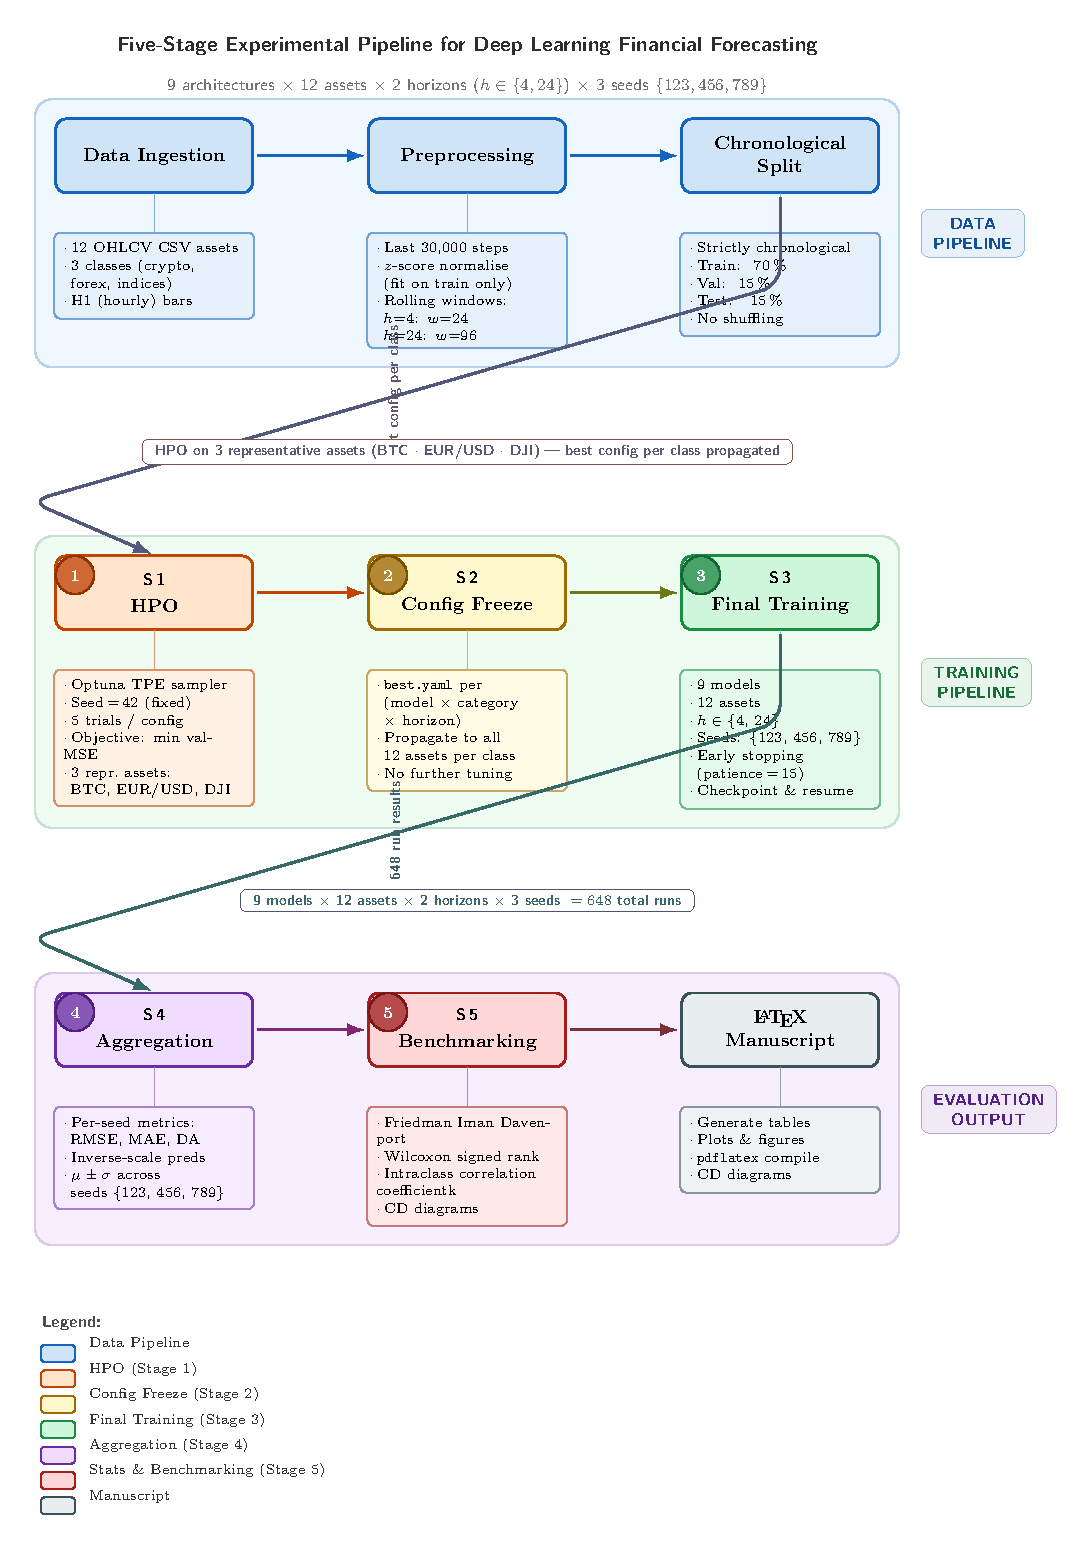
\includegraphics[width=\textwidth]{figures/02_pipeline_diagram.pdf}
  \caption{Five-stage experimental pipeline.  \textbf{Stage~1:} Fixed-seed Bayesian HPO on representative assets (BTC/USDT, EUR/USD, Dow Jones; seed~42; \ntrials Optuna TPE trials; 50~epochs per trial).  \textbf{Stage~2:} Best configuration frozen per (model, category, horizon) triple.  \textbf{Stage~3:} Multi-seed final training (seeds 123, 456, 789; 100~epochs maximum; early stopping with patience~15).  \textbf{Stage~4:} Test-set metric aggregation with inverse scaling (mean~$\pm$~std across seeds).  \textbf{Stage~5:} Benchmarking with rank-based leaderboard analysis, visualisation, and variance decomposition.  All 918 experimental runs---270 HPO trials plus 648 final training runs---are conducted under identical conditions.}
  \label{fig:pipeline}
\end{figure}

% --------------------------------------------------------------------------
\subsection{Evaluation Metrics}
\label{sec:metrics}

Three complementary metrics are computed on the held-out test set for every (model, asset, horizon, seed) configuration.  All predictions are inverse-transformed to the original price scale before computation, ensuring that error magnitudes are economically interpretable.

\begin{enumerate}[nosep]
  \item \textbf{\rmse (Root Mean Squared Error)}---the \emph{primary ranking metric}, penalising large deviations quadratically.  \rmse is appropriate for financial risk assessment, where large forecast errors carry disproportionate cost:
  \begin{equation}
    \text{RMSE} = \sqrt{\frac{1}{n}\sum_{i=1}^{n}(y_i - \hat{y}_i)^2}.
    \label{eq:rmse}
  \end{equation}

  \item \textbf{\mae (Mean Absolute Error)}---a secondary metric that is robust to outliers and provides a median-biased point estimate of forecast error:
  \begin{equation}
    \text{MAE} = \frac{1}{n}\sum_{i=1}^{n}|y_i - \hat{y}_i|.
    \label{eq:mae}
  \end{equation}

  \item \textbf{\da (Directional Accuracy)}---the fraction of horizon steps where the predicted direction of price change matches the realised direction, providing an economically interpretable measure of forecast quality relevant to trading-signal applications:
  \begin{equation}
    \text{DA} = \frac{1}{n}\sum_{i=1}^{n}\mathbb{1}\!\left[\text{sign}(\hat{y}_i - \hat{y}_{i-1}) = \text{sign}(y_i - y_{i-1})\right].
    \label{eq:da}
  \end{equation}
\end{enumerate}

All results are reported as mean~$\pm$~standard deviation across \nseeds seeds (123, 456, 789), enabling quantification of initialisation-induced uncertainty.  The concordance between \rmse and \mae rankings is examined in Section~\ref{sec:category_analysis} to verify that findings are robust to the choice of error metric.

% --------------------------------------------------------------------------
\subsection{Statistical Validation Framework}
\label{sec:statistical_framework}

A two-tier framework is employed to characterise observed performance differences:

\begin{enumerate}[nosep]
  \item \textbf{Two-factor variance decomposition} $\rightarrow$ \textbf{H3}.  A sum-of-squares decomposition partitions total forecast variance into three components: model-attributable, seed-attributable, and residual interaction.  Reported as a percentage of total sum of squares across three panels (raw, z-normalised all models, z-normalised modern only).

  \item \textbf{Spearman rank correlation} $\rightarrow$ \textbf{H2, H4}.  Spearman's $\rho$ between $\hfour$ and $\htwentyfour$ model rankings per asset tests cross-horizon stability (H2).  Spearman's $\rho$ between parameter count and mean \rmse rank tests whether complexity--performance is monotonic (H4).  Both correlations are tested for significance against $\rho = 0$.
\end{enumerate}

% --------------------------------------------------------------------------
\subsection{Experimental Scale}
\label{sec:experimental_scale}

The total experimental scale is:

\begin{itemize}[nosep]
  \item \textbf{HPO (Stage~1):} $9 \text{ models} \times 3 \text{ representative assets} \times 2 \text{ horizons} \times 5 \text{ trials} = 270$ trial runs.
  \item \textbf{Final training (Stage~3):} $9 \text{ models} \times 12 \text{ assets} \times 2 \text{ horizons} \times 3 \text{ seeds} = 648$ training runs.
  \item \textbf{Total:} $270 + 648 = \mathbf{918}$ experimental runs.
\end{itemize}

Each of the 648 final training runs produces a separate metrics evaluation on the test set, yielding 648 individual (model, asset, horizon, seed) performance records that form the basis of all analyses in Section~\ref{sec:results}.
